\newpage
\section{El problema}\label{sec:problema}

Un yacimiento petrol\'\i fero es una acumulaci\'on natural de hidrocarburos (gas natural y petr\'oleo, entre otros) en el subsuelo. Debido a la creciente escasez de reservas de hidrocarburos acumulados en yacimientos convencionales, la industria del petr\'oleo y diversos gobiernos nacionales han tornado su atenci\'on en las \'ultimas d\'ecadas a la explotaci\'on de yacimientos no convencionales. Uno de los tipos de yacimientos m\'as explorados est\'a dado por las reservas de petr\'oleo y gas natural almacenados en un tipo de rocas sedimentarias llamadas pelitas (shale), conocidos como yacimientos de \emph{shale gas} y \emph{shale oil}.
 
La explotaci\'on de este tipo de yacimientos utiliza m\'etodos de fractura hidr\'aulica, por medio de los cuales se generan fracturas en la roca madre para concentrar el petr\'oleo y el gas natural y posteriormente proceder a su extracci\'on. A pesar de que las primeras inyecciones de material para la extracci\'on de hidrocarburos se remontan a la segunda mitad del siglo XIX, reci\'en se comenz\'o a usar este tipo de m\'etodos en forma extensiva a prin\-ci\-pios del siglo XXI, principalmente en Estados Unidos. Adem\'as de las reservas en Estados Unidos, en la \'ultima d\'ecada se han descubierto enormes reservas de shale gas y shale oil en Argentina, Canad\'a y China.

Se describe el proceso de explotaci\'on de un yacimiento \emph{shale}. En primer lugar, se realizan varias perforaciones verticales en el subsuelo que llegan hasta la roca madre. Como se ve a continuaci\'on:

\begin{center}
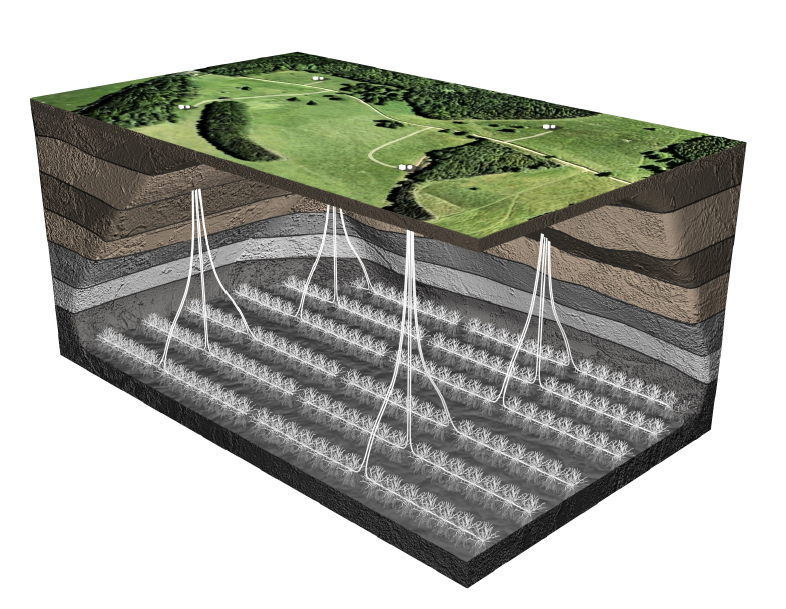
\includegraphics[width=0.6\textwidth]{imagenes/figura1}
\end{center}

El sector en la superficie alrededor de las bocas de pozo se denomina locaci\'on, y habitualmente ocupa un \'area rectangular de entre algunas decenas y unos pocos cientos de metros por lado. Estos equipos son los \'unicos que se ven en la superficie, y habitualmente su instalaci\'on involucra obras de nivelaci\'on del suelo y construcci\'on de caminos de acceso. Como consecuencia, las locaciones no pueden estar sobre cursos de agua, barrancos o en sitios montanosos.

\begin{center}
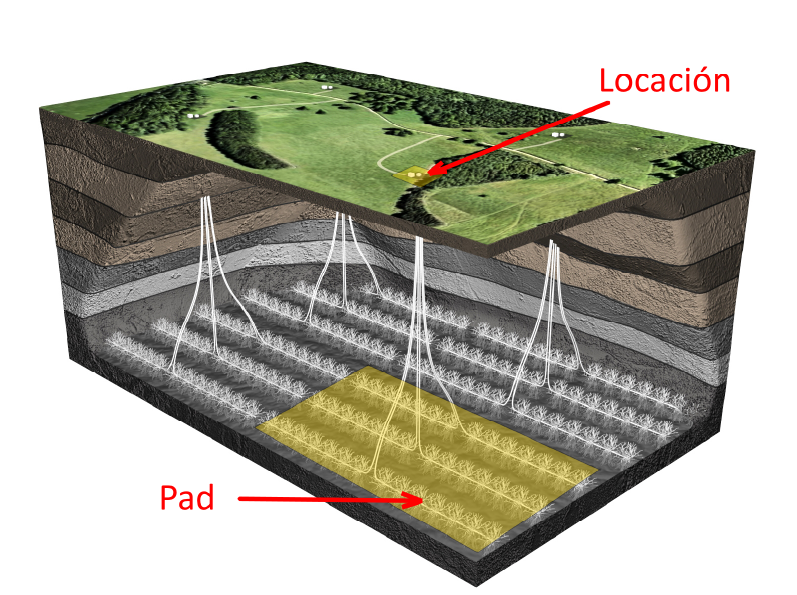
\includegraphics[width=0.45\textwidth]{imagenes/figura2}
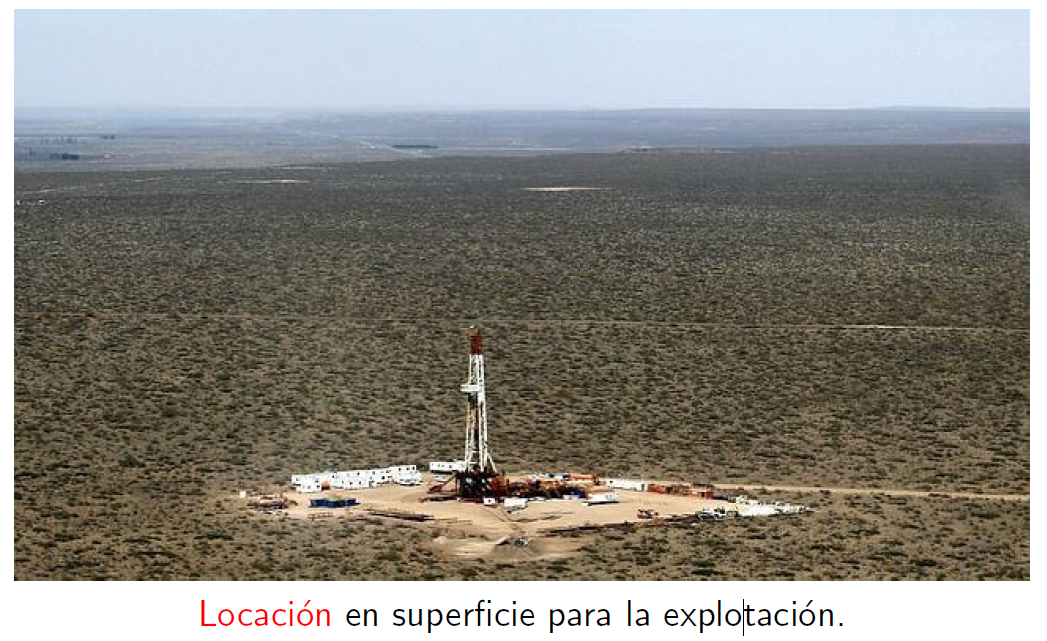
\includegraphics[width=0.45\textwidth]{imagenes/figura3}
\end{center}

Cada perforaci\'on atraviesa la roca madre, y a lo largo de esta perforaci\'on
se realizan los procesos de inyecci\'on de materiales para lograr la fractura de
la roca. Luego, se utilizan las mismas para la extracci\'on de los hidrocarburos
que migran hacia las zonas de fractura.

La zona
explotada a partir de una locaci\'on se denomina pad, y tiene una forma t\'ipicamente
rectangular.

Dadas estas caracter\'isticas del problema queremos que las zonas de fractura en la roca madre no se deban superponer.


Al momento de planificar la explotaci\'on de un yacimiento no convencional,
uno de los principales problemas a resolver es donde ubicar las locaciones y
que tipo de explotaci\'on realizar en cada una (lo cual determina el tipo y
tamano de los pads resultantes) con el objetivo de maximizar la producci\'on
y minimizar los costos y el impacto ambiental. Este problema se conoce con
el nombre de optimizaci\'on del \'area de drenaje, y como resultado se espera un
plan de explotaci\'on que muestre las ubicaciones de locaciones y pads.


En la siguiente figura podemos ver  el mapa de un yacimiento, y las configuraciones de pads que
podemos usar para la explotaci\'on.

\begin{center}
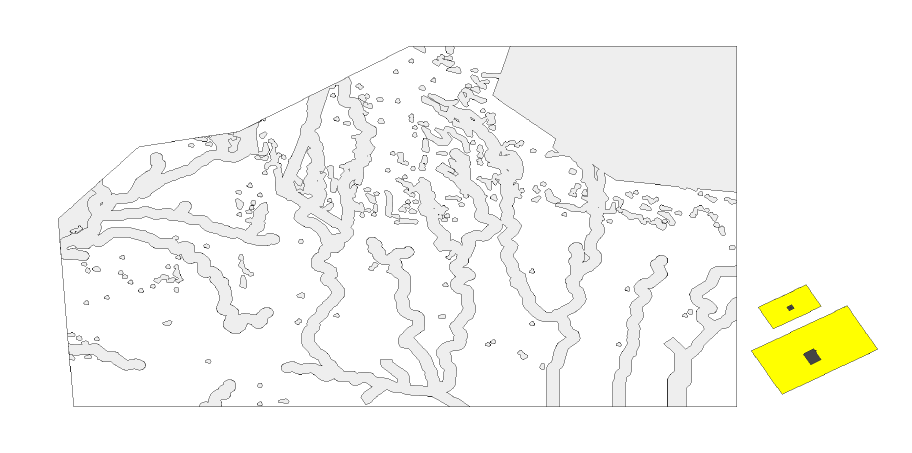
\includegraphics[width=0.6\textwidth]{imagenes/figura4}
\end{center}

Los pads se deben ubicar siguiendo cierto \'angulo $\alpha$, llamado direcci\'on de esfuerzo horizontal m\'inimo.
Como por ejemplo:

\begin{center}
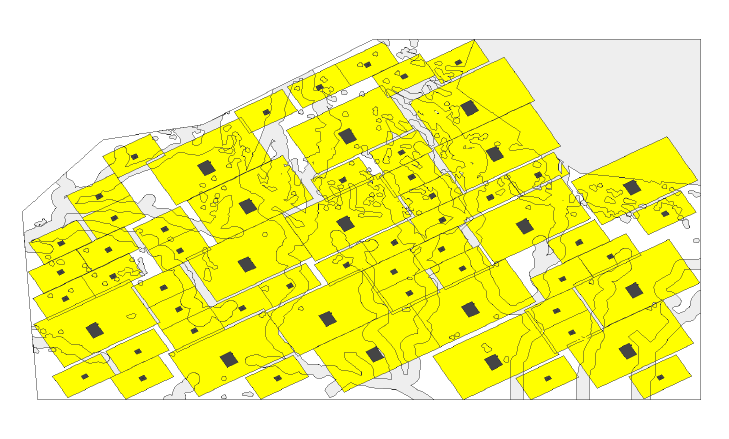
\includegraphics[width=0.45\textwidth]{imagenes/figura5}
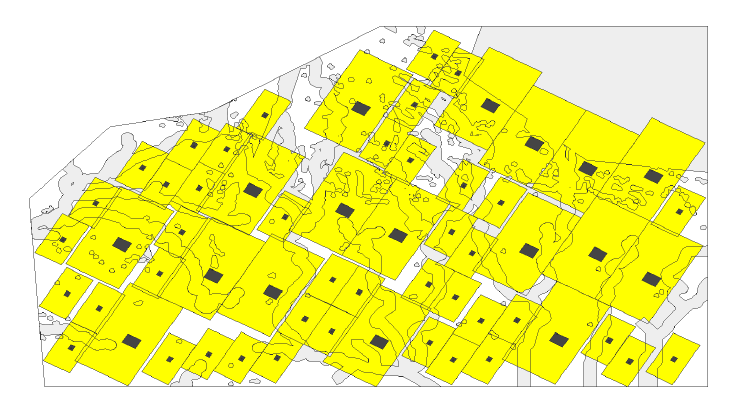
\includegraphics[width=0.45\textwidth]{imagenes/figura6}
\end{center}

Formalmente, los datos de entrada del problema est\'an dados por los siguientes
elementos:

\begin{enumerate}
\item El yacimiento Y  $\subseteq$ $\mathbb{R}^2$, que en este trabajo asumimos dado por un pol\'igono en el plano (no necesariamente convexo). Todos los pads deben estar ubicados dentro del per\'imetro del yacimiento.
\item Una funci\'on ogip : Y $\rightarrow \mathbb{R}_{+}$ (original gas in place), que especifica la
cantidad de shale gas esperada en cada punto del yacimiento, y el precio
de venta $\rho  \in \mathbb{R}_{+}$ de cada unidad extra\'ida. 

Dado un pad P $\subseteq$ Y ubicado
dentro del yacimiento, el gas total obtenido por explotar el pad esta dado
por ogip(P) := $\int_{P}^{} ogip(x) dx$
\item Un conjunto S = \{$S_1$,...,$S_k$\} de configuraciones posibles de pads, que
podemos utilizar para explotar el yacimiento. Para cada configuraci\'on S $\in$ S, tenemos estos datos:
\begin{enumerate}
\item  Largo $lp_S \in \mathbb{R}_{+}$ y ancho $ap_S \in \mathbb{R}_{+}$ del pad, en metros.
\item  Largo $ll_S \in \mathbb{R}_{+}$ y ancho $al_S \in \mathbb{R}_{+}$ de la locaci\'on en metros, y asumimos que $ll_S < lp_S$ y $al_S < ap_S$.
\item  La locaci\'on esta ubicada en el centro del pad, pero se puede mover algunos metros de este centro para evitar obst\'aculos geogr\'aficos. El par\'ametro de tolerancia $tol_S \in \mathbb{R}_{+}$ especifica la cantidad m\'axima de metros que el centro de la locaci\'on se puede mover con relaci\'on
al centro del pad.
\item  Finalmente, se tiene el costo $c_S \in \mathbb{R}_{+}$ de construcci\'on del pad.
Dado un pad P correspondiente a la configuraci\'on S, definimos su margen neto como $neto(P) := \rho$ X $ogip(P) - c_S$.
\end{enumerate}
\item  Un conjunto de obst\'aculos (habitualmente de \'indole geogr\'afica) que las locaciones deben evitar. Consideramos que cada obst\'aculo esta dado por un pol\'igono en el plano, y ninguna locaci\'on se puede superponer con ning\'un obst\'aculo.
\item Un \'angulo $\alpha \in [0; 2\pi]$ de explotaci\'on ideal, denominado \'angulo de esfuerzo horizontal m\'inimo, que especifica la orientaci\'on aproximada que deben tener los pozos horizontales sobre el yacimiento con relaci\'on al norte geogr\'afico. Como esta orientaci\'on es aproximada, se tiene una tolerancia $\beta \in [0; 2\pi]$, que especifica que todos los pads deben estar orientados en un \'angulo comprendido en el intervalo $[\alpha - \beta, \alpha + \beta]$.
\end{enumerate}



El problema consiste en hallar un conjunto de pads Ps = \{$P_1, ... ,P_n$\} y un conjunto de locaciones Ls = \{$L_1, ..., L_n$\} (de modo tal que la locaci\'on $L_i$ corresponde al pad $P_i$, para i = 1,...,n) que maximice $neto(P) :=  \sum_{i=1}^{n} neto(P_i) $ de modo tal que se cumplan las siguientes restricciones:

\begin{enumerate}
\item Todos los pads deben estar contenidos dentro del yacimiento, es decir $P_i \subseteq Y$ para i = 1,...,n.
\item Como restricci\'on, los pads de la soluci\'on no se deben superponer, dado que corresponden a zonas de fractura en la roca madre.
\item Cada pad y su locaci\'on deben responder a las especificaciones de una conguraci\'on de S. Es decir, para cada i = 1,...,n debe existir una configuraci\'on S $\in$ S tal que $P_i$ tiene largo $lp_S$ y ancho $ap_S$, $L_i$ tiene largo $ll_S$ y ancho $al_S$ y su centro esta a no m\'as de $tol_S$ metros del centro de $P_i$, y finalmente $P_i$ y $L_i$ est\'an orientados en un mismo \'angulo, el cual debe estar entre $[\alpha - \beta, \alpha + \beta]$.
\item Ninguna locaci\'on de Ls se debe superponer con ning\'un obst\'aculo.
\end{enumerate}


Por ejemplo, en la siguiente figura se muestra un yacimiento y los obst\'aculos dentro del yacimiento, y en la figura contigua se muestra una soluci\'on factible para $\alpha = \pi / 4$ y para dos configuraciones posibles. Dado que la funci\'on ogip no siempre esta bien determinada de antemano (y en ocasiones se trabaja con estimaciones poco fiables de esta funci\'on) alternativamente se puede solicitar que se maximice el \'area total cubierta con los pads propuestos, en lugar del beneficio neto total obtenido. El algoritmo que se presenta en la pr\'oxima secci\'on permite utilizar cualquiera de estas dos funciones objetivo, o una combinaci\'on lineal de ambas.



\begin{center}
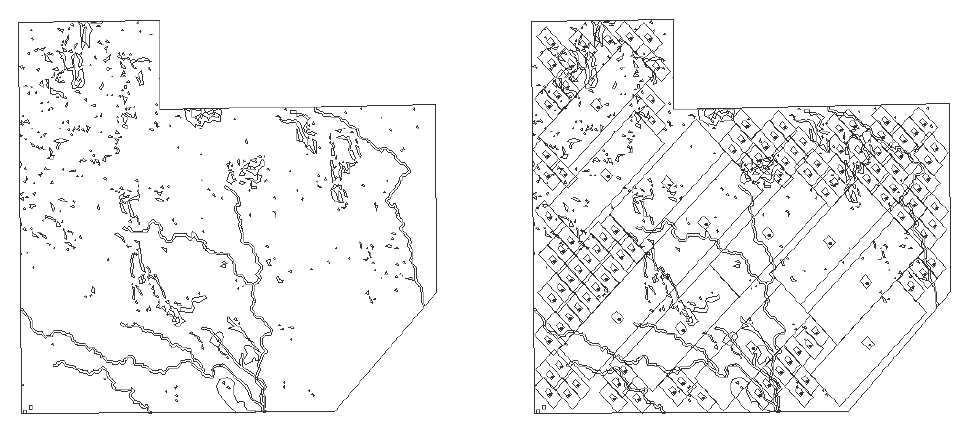
\includegraphics[width=1\textwidth]{imagenes/figura7}
\end{center}



